\documentclass[11pt,twoside]{article}
\usepackage{style}

\begin{document}
  \title{EVA}
  \author{The CodeAnon Organization}

  \maketitle
  \begin{abstract}
    We propose in this paper a virtual machine made for students, designed and implemented by students, to facilitate learning low-level programming. The virtual machine, while simple, is feature-complete, allowing users to run applications of all sizes on top of it.
  \end{abstract}
  \vfill
  \begin{center}
    
\includegraphics[height=8cm]{logo_graph.pdf}
  \end{center}
  \vfill

  \cleardoublepage

  \hspace{0pt}
  \vfill

  \section*{Preliminary remarks}

  This document, while written in the present tense, is a mere projection of what \noun{Eva} will eventually become. This document is therefore a detailled description of the final version of \noun{Eva} and not a description of its current state. Moreover, changes to this document will eventually be made during the development of the project.

  \vfill

  \clearpage

  \tableofcontents
  \cleardoublepage

  \hspace{0pt}
  \vfill

  \section{Introduction}

  Assembler is the first abstraction into programmable circuits. As such, learning it is a fundamental step for the student curious to peel off the layers of engineering behind the computer. Moreover, many other fields of computer science need a deep knowledge of assembly languages; for example writing a compiler relies upon knowing about the different architectures around today (ARM, x86, PowerPC, etc.) and of the assembly languages associated to them.

  Therefore, how can we allow students willing to try themselves at this kind of practice to complete their projects? Faced with the number of architectures to target, and to the complexity of some of them, this kind of project can quickly become unbearable for a student to take on.\\
  Alternatives, of course, already existes. We can cite the infamous book \emph{Structure And Interpretation of Computer Programs}\cite{SICP}, which proposes in its last chapter the implementation of an ``abstract machine'' programmable in a simple assembly language. Other projects, like the virtual machine \noun{CHIP8} are interesting sources to discover assembly programming\cite{CHIP8}. These tools are already used with the goal of making ``low-level'' accessible to students, but nevertheless stay very specific and greatly limit the range of possibilities they offer.

  It's at this crossroad between \emph{easy to learn} and \emph{range of possibilities} that the project lies; the void between teaching tools and real-world problems that \noun{Eva} tries to fill.

  \section{Existing projects}

  Other virtual machines exist like the \emph{Java Virtual Machine}, or the \emph{Common Language Runtime}, which are designed as generalist VMs. These are both performance-oriented and feature-complete; but as a result, they are complex and oftentimes impossible to tackle by students.

  \vfill
  \newpage

  \section{Project description}

  \noun{Eva} is a light virtual machine made by students, for students. Its simplicity offers grounds for experimentation well-tailored to teach assembly programming, or related concepts like compilation. Because \noun{Eva} is open-source, students can peek into the core of the machine to better understand it. It also means that people can easily modify it, for experimentation or to make it better.\\
  \noun{Eva} is programmable with a short, but complete instruction set; by that we mean that the instruction set is ``complete enough to allow applications of a decent size, including I/O, graphical output and possibly networking''. We dive in deeper into this later in the document.

  \subsection{Technical description}

  The entierty of the \noun{Eva} project is composed of several tools, as shown in \figref{diagram1}.
  \begin{figure}[tb]
    \centering
    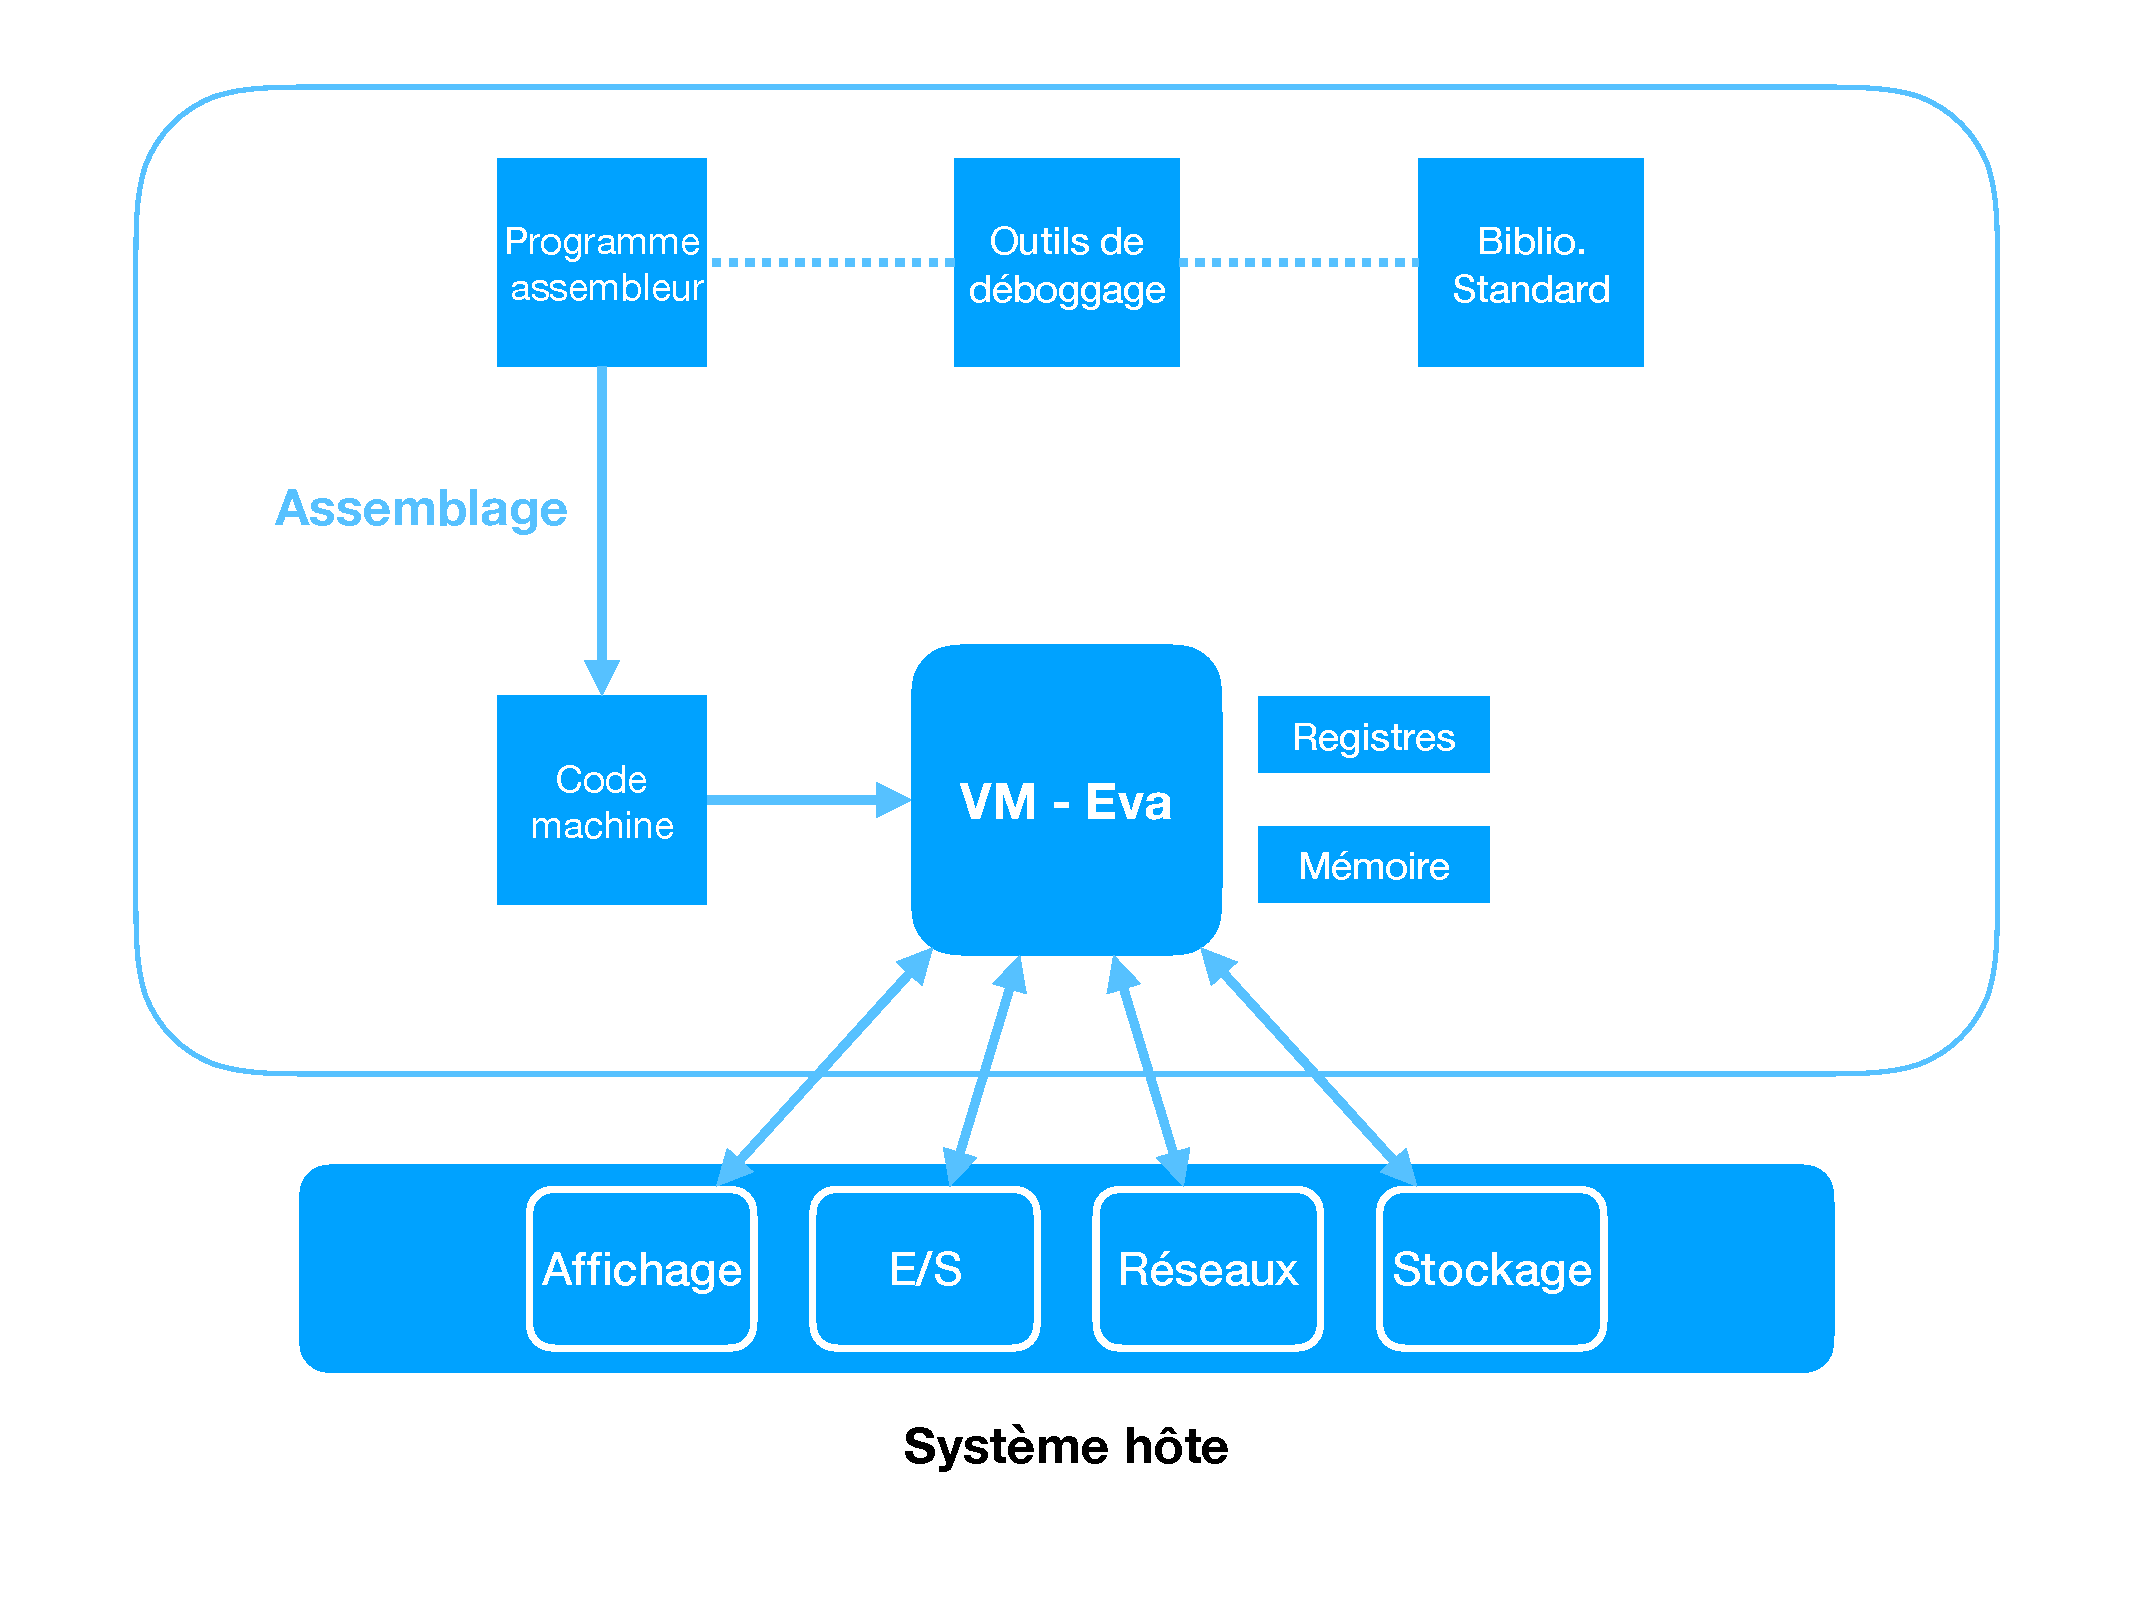
\includegraphics[width=12cm, height=12cm, keepaspectratio]{diagram1_graph.pdf}
    \caption{Structure de la machine virtuelle \noun{Eva}}
    \label{fig:diagram1}
  \end{figure}

  \begin{itemize}
    \item[VM Core] \noun{Eva}'s machine language interpreter. It's this program that interfaces between the user and the (physical) machine.
    \item[Assembly \noun{Eva}] This tool converts assembly code into an executable made for \noun{Eva}. It also includes a linker allowing an \noun{Eva} program to be written in several modules.
    \item[Debugging tool] Allows users, while writing code for \noun{Eva}, to debug their program, by showing memory contents, and observe in detail how their program behaves when executed in the virtual machine. This tool can also manipulate the memory of the executing program.
    \item[Standard library] This module contains utility and math functions to be made available for \noun{Eva} programs. This module can be explicitely loaded in memory before execution of the program and used through system calls. Another alternative is to use the linker above to link the standard library in order to bundle the module into the executable.
  \end{itemize}

  \subsection{Elements of design}

  The virtual machine needs to be minimalist in order to be accessible to students wanting to learn about the project or the subject in general, but also needs adequate performance to support larger-scale applications. \noun{Eva} being developed with a ``return to fundamentals'', its development is minimalist and only brings what's essential by offering an instruction set that's concise and simple. To this end, we selected an instruction set based on a subset of the ARM instruction set, shown in \tabref{instructions}.

  \begin{table}
    \begin{centering}
      \begin{tabular}{|c|l|}
        \hline
      \textbf{Instruction} & \textbf{Description}                \\
      \hline
      \hline
      \textbf{ADD}         & Addition                            \\
      \hline
      \textbf{ADC}         & Addition with carry               \\
      \hline
      \textbf{BIC}         & Bit reset                          \\
      \hline
      \textbf{CMP}         & Comparison                         \\
      \hline
      \textbf{MOV}         & Move \\
      \hline
      \textbf{B}           & Branch Jump                \\
      \hline
      \textbf{BL}          & Branch Link                  \\
      \hline
      \textbf{PUSH}        & Enqueue                             \\
      \hline
      \textbf{POP}         & Dequeue                             \\
      \hline
      \textbf{SUB}         & Subtraction with carry           \\
      \hline
      \end{tabular}
    \end{centering}
    \caption{Instruction set supported by \noun{Eva}}
    \label{tab:instructions}
  \end{table}

  \subsection{\noun{Eva}'s virtual machine implementation}

  In order to aid with development, \noun{Eva} will be written in C99 and should not have any dependency beyond the standard library. Such a constraint enforces a clear implementation and the portability of the project's source code.

  This minimalist implementation goes hand in hand with \noun{Eva}'s ideology: Prioritize accessibility and reliability. Furthermore, the security aspect is important for the project, and code correction will always have the priority over implementing new functionality and features.

  \subsection{Disponibility}

  \noun{Eva} is an open-source project, where its source code and binaries will be available under an MIT license. This means anybody is allowed to read, download, and modify the source code. As an educational project, we believe it is only natural that the project be made publicly available for the greatest amount of people.

  \section{Related projects}

  On top of its development, several other projects maintained by the team will build off of \noun{Eva}, including everal compilers targeting \noun{Eva}, and a high-level programming language that will complement the assembly langauge natively supported by the virtual machine.

  \section{Usage exemples}

  In this sections, we present several useful scenarios of usage of \noun{Eva}:

  \begin{itemize}
    \item \textbf{Assembly of a file} \texttt{evasm -a source.evasm -o main.evo}
    \item \textbf{Assembly and linking of a single source file} \texttt{evasm source.evasm -o main.eva}
    \item \textbf{File execution} \texttt{evasm -l module1.evo module2.evo source.evo -o main.eva}
    \item \textbf{File execution} \texttt{eva main.eva}
    \item \textbf{File execution with debug} \texttt{eva main.eva --debug}
    \item \textbf{File execution with memory limit} \texttt{eva main.eva --ram 200}
    \item \textbf{File execution with explicit loading of stdlib} \texttt{eva main.eva --std}
  \end{itemize}

  \cleardoublepage

  \begin{thebibliography}{XXXXXX}
	\label{chap:bib}

	\bibitem{SICP} Harold Abelson and Gerald Jay Sussman
	\emph{Structure and Interpretation of Computer Programs} MIT, 1996

	\bibitem{CHIP8} Joseph Weisbecker
	\emph{CHIP-8 programming language and virtual machine} 1978

\end{thebibliography}

\end{document}
